\documentclass[11pt]{article}
\usepackage{geometry, titlesec}
\usepackage[parfill]{parskip}
\usepackage[italicdiff]{physics}
\usepackage{amsfonts, amsthm}
\usepackage[cm]{fullpage}
\usepackage{fancyhdr}
\usepackage{enumitem}
\usepackage{xcolor, soul}
\usepackage{graphicx}
\usepackage[export]{adjustbox}
\usepackage{siunitx}
%\allowdisplaybreaks

\renewcommand{\thesubsection}{\thesection.\alph{subsection}}
\setenumerate[1]{label={(\alph*)}}

\makeatletter
\renewcommand*\env@cases[1][1.2]{%
  \let\@ifnextchar\new@ifnextchar
  \left\lbrace
  \def\arraystretch{#1}%
  \array{@{}l@{\quad}l@{}}%
}
\makeatother
 
\renewcommand{\footrulewidth}{.2pt}
%\setlist[enumerate]{leftmargin=*}
\pagestyle{fancy}
\fancyhf{}
\rhead{Physics 132-B}
\lhead{\textbf{Homework 5 Solutions}}
%\rhead{A--De Discussion}
\setlength{\headheight}{11pt}
\setlength{\headsep}{11pt}
\setlength{\footskip}{24pt}
\lfoot{\today}
\rfoot{\thepage}

\titleformat{\subsection}[runin]{\normalfont\large\bfseries}{\thesubsection}{1em}{}
\newcommand{\refeq}[1]{(\ref{#1})}

\newcommand{\beq}{\begin{equation*}}
\newcommand{\eeq}{\end{equation*}}

\newcommand{\beqn}{\begin{equation}}
\newcommand{\eeqn}{\end{equation}}

\newcommand{\blg}{\begin{align*}}
\newcommand{\elg}{\end{align*}}

\makeatletter
\renewcommand*\env@matrix[1][*\c@MaxMatrixCols c]{%
  \hskip -\arraycolsep
  \let\@ifnextchar\new@ifnextchar
  \array{#1}}
\makeatother


\newenvironment{statement}
{
%    \color{gray}
    \ignorespaces
}
{
%    \smallskip
}

\newenvironment{problem}
{
    \color{darkgray}
    \ignorespaces
}

\newenvironment{solution}
{
    \paragraph{Solution.}
    \ignorespaces
}
{
    \bigskip
}

\renewcommand{\vec}[1]{\mathbf{#1}}
\renewcommand{\theequation}{\Alph{equation}}


\begin{document}

\newcommand{\Vab}{V_{ab}}
\newcommand{\cE}{\mathcal{E}}
\newcommand{\sicE}{\SI{12.0}{\volt}}
\newcommand{\sir}{\SI{0.40}{\ohm}}
\newcommand{\siP}{\SI{80.0}{\watt}}
	

\paragraph{Problem 25.58}
\begin{problem}
	A resistor with resistance $R$ is connected to a battery that has emf {\sicE} and internal resistance $r = \sir$.  For what two values of $R$ will the power in the resistor be {\siP}?
\end{problem}

\begin{solution}
	The power $P$ delivered to a resistor is
	\beqn \tag{25.18} \label{25.18}
		P = I^2 R,
	\eeqn
	where $I$ is the current through the resistor and $R$ its resistance.  We can find the current from
	\beqn \tag{25.17} \label{25.17}
		\Vab = \cE - I r,
	\eeqn
	where $\Vab$ is the voltage difference across the resistor, $\cE$ is the emf of the battery, and $r$ its internal resistance.  We also know that
	\beqn \tag{25.11} \label{25.11}
		\Vab = I R.
	\eeqn
	Substituting \refeq{25.11} into \refeq{25.17}, we get
	\beq
		IR = \cE - Ir
		\implies
		\cE = I (R + r)
		\implies
		I = \frac{\cE}{R + r}.
	\eeq
	Now we can substitute this result into \refeq{25.18} and solve for $R$:
	\begin{align*}
		P = \frac{\cE^2}{(R + r)^2} R
		&\implies
		\cE^2 R = P (R^2 + 2 R r + r^2)
		\implies
		0 = P R^2 + (2P r - \cE^2) R + P r^2 \\
		&\implies
		R = \frac{\cE^2 - 2 P r \pm \sqrt{(2P r - \cE^2)^2 - 4 P^2 r^2}}{2 P}
	\end{align*}
	Plugging in our numerical values for $r$, $P$, and $\cE$, and recalling that $\SI{1}{\watt} = \SI{1}{\square\volt\per\ohm}$, we get
	\begin{align*}
		R &= \frac{(\sicE)^2 - 2 (\siP) (\sir) \pm \sqrt{[2 (\siP) (\sir) - (\sicE)^2]^2 - 4 (\siP)^2 (\sir)^2}}{2 (\siP)} \\
		&= \frac{\SI{80.0}{\square\volt} - \pm \sqrt{(\SI{80}{\square\volt})^2 - (\SI{64}{\square\volt})}}{\SI{160}{\square\volt\per\ohm}}
		= \frac{\SI{80.0}{\square\volt} \pm \sqrt{\SI{2306}{\volt^4}}}{\SI{160}{\square\volt\per\ohm}}
		= \frac{80.0 \pm 48.0}{160} \,\si{\ohm}
		= (0.50 \pm 0.30) \,\si{\ohm}.
	\end{align*}
	So the two possible resistances are
	{\color{blue} \begin{align*}
		R &= \SI{0.80}{\ohm}, &
		R &= \SI{0.20}{\ohm}.
	\end{align*}}
\end{solution}

\clearpage



\newcommand{\Iq}{I_1}
\newcommand{\Iw}{I_2}
\newcommand{\Ie}{I_3}
\newcommand{\Sohm}[1]{\SI{#1}{\ohm}}
\newcommand{\Svolt}[1]{\SI{#1}{\volt}}
\newcommand{\Samp}[1]{\SI{#1}{\ampere}}

\begin{minipage}[l]{0.7\textwidth}
\paragraph{Exercise 26.26}
\begin{problem}
	In the circuit shown in \textbf{Fig.~E26.26}, find \medskip
	\begin{enumerate}
		\item the current in each branch, and \medskip
		\item the potential difference $\Vab$ of point $a$ relative to point $b$.
	\end{enumerate}
\end{problem}
\end{minipage}%
\hspace{0.05\textwidth}%
\begin{minipage}{0.25\textwidth}
	\center 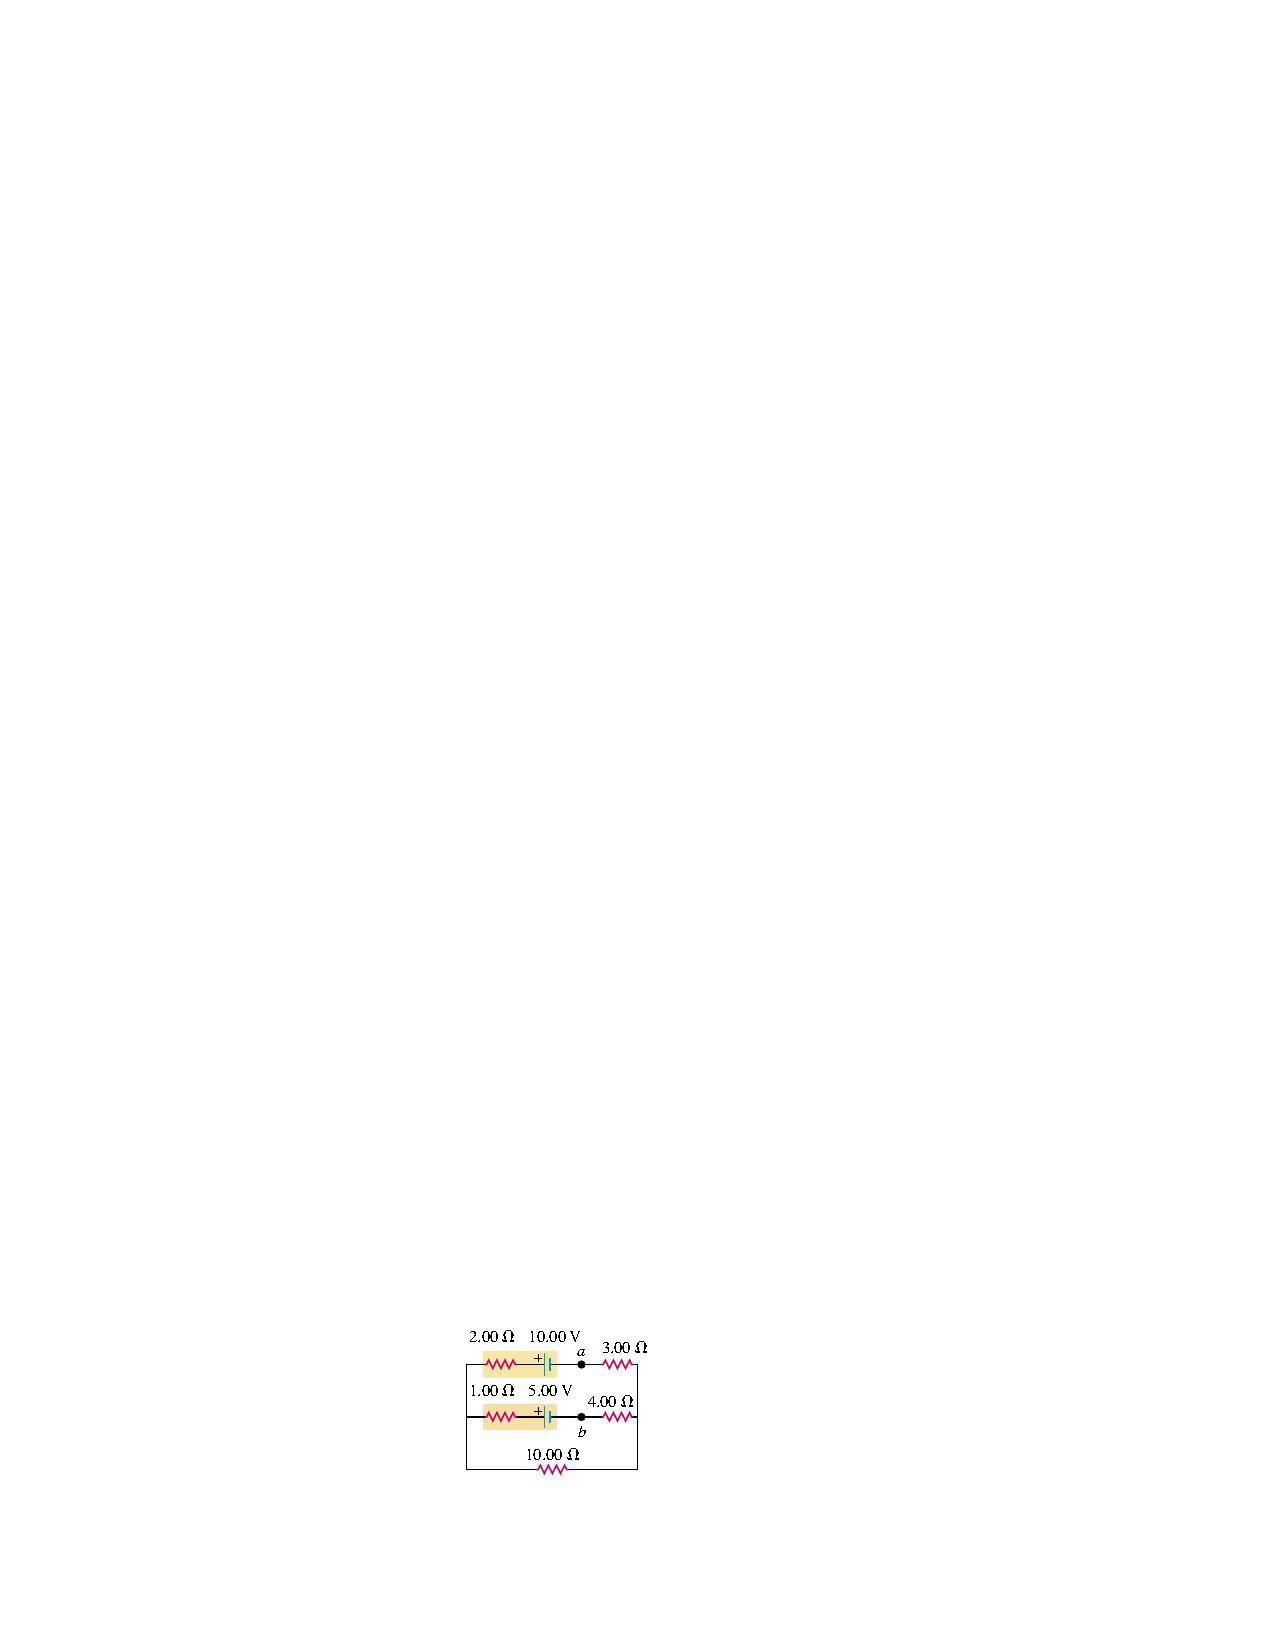
\includegraphics[scale=1.25]{E26-26}
	\center \textbf{Figure E26.26}
\end{minipage}


\begin{solution}
 	For this problem we need to use Kirchhoff's rules:
	\begin{align}
		\sum I &= 0 & &\text{(junction rule)}, \tag{26.5} \label{26.5} \\
		\sum V &= 0 & &\text{(loop rule)}. \tag{26.6} \label{26.6}
	\end{align}
	
	\begin{enumerate}
		\item Let $\Iq$ be the current through the top branch, $\Iw$ the current through the middle branch, and $\Ie$ the current through the bottom branch.  Let's choose all three currents to be flowing to the left.  Then applying the junction rule to the junction on the left gives us
		\beq
			0 = \Iq + \Iw + \Ie.
		\eeq
		Now we will apply the loop rule to the top and the bottom loops, and move through each counterclockwise, starting at the battery.  For the top loop,
		\beq
			0 = \Svolt{10} - (\Sohm{2}) \Iq + (\Sohm{1}) \Iw - \Svolt{5} + (\Sohm{4}) \Iw - (\Sohm{3}) \Iq
			\implies
			\Svolt{5} = (\Sohm{5}) \Iq - (\Sohm{5}) \Iw
			\implies
			\Samp{1} = \Iq - \Iw,
		\eeq
		where in going to the final equation we have simply divided by $\Sohm{5}$, since $\SI{1}{\volt} = \SI{1}{\ohm\ampere}$.  For the bottom loop,
		\beq
			0 = \Svolt{5} - (\Sohm{1}) \Iw + (\Sohm{10}) \Ie - (\Sohm{4}) \Iw
			\implies
			\Svolt{5} = (\Sohm{5}) \Iw - (\Sohm{10}) \Ie
			\implies
			\Samp{1} = \Iw - 2 \Ie.
		\eeq
		Now we have three equations in three unknowns, which you can solve using your favorite method.  I like to do Gaussian elimination with an augmented matrix.  The matrix equation is
		\beq
			\mqty[ 1 & 1 & 1 \\
				1 & -1 & 0 \\
				0 & 1 & -2 ]
				\mqty[ \Iq \\ \Iw \\ \Ie ]
				= \mqty[ 0 \\ 1 \\ 1 ],
		\eeq
		which can be solved as follows:
		\begin{align*}
			\begin{bmatrix}[c c c | c]
				1 & 1 & 1 & 0 \\
				1 & -1 & 0 & 1 \\
				0 & 1 & -2 & 1
			\end{bmatrix}
			&\sim
			\begin{bmatrix}[c c c | c]
				1 & -1 & 0 & 1 \\
				0 & 1 & -2 & 1 \\
				1 & 1 & 1 & 0
			\end{bmatrix}
			\sim
			\begin{bmatrix}[c c c | c]
				1 & 0 & -2 & 2 \\
				0 & 1 & -2 & 1 \\
				0 & 2 & 1 & -1
			\end{bmatrix}
			\sim
			\begin{bmatrix}[c c c | c]
				1 & 0 & -2 & 2 \\
				0 & 1 & -2 & 1 \\
				0 & 0 & 5 & -3
			\end{bmatrix}
			\sim
			\begin{bmatrix}[c c c | c]
				1 & 0 & -2 & 2 \\
				0 & 1 & -2 & 1 \\
				0 & 0 & 1 & -3/5
			\end{bmatrix} \\
			&\sim
			\begin{bmatrix}[c c c | c]
				1 & 0 & 0 & 4/5 \\
				0 & 1 & 0 & -1/5 \\
				0 & 0 & 1 & -3/5
			\end{bmatrix}.
		\end{align*}
		So we have {\color{blue}
		\begin{align*}
			\Iq &= \Samp{0.800} \text{ (to the left)}, &
			\Iw &= -\Samp{0.200} \text{ (to the right)}, &
			\Ie &= -\Samp{0.600} \text{ (to the right)}.
		\end{align*}}
		
		\item We can find the potential difference between points $a$ and $b$ by moving counterclockwise through the top loop, similar to applying the loop rule in (a).  But now we start at $b$ and end on $a$:
		\beq
			\Vab = (\Sohm{4}) \Iw - (\Sohm{3}) \Iq
			= (\Sohm{4.00}) (-\Samp{0.200}) - (\Sohm{3.00}) (\Samp{0.800})
			= {\color{blue} \Svolt{32.0}}.
		\eeq
	\end{enumerate}
\end{solution}



\clearpage

\begin{minipage}[l]{0.65\textwidth}
\paragraph{Exercise 26.29}
\begin{problem}
	In the circuit shown in \textbf{Fig.~E26.29} the batteries have negligible internal resistance and the meters are both idealized.  With the switch $S$ open, the voltmeter reads \SI{15.0}{\volt}. \medskip
	\begin{enumerate}
		\item Find the emf $\cE$ of the battery. \medskip
		\item What will the ammeter read when the switch is closed?
	\end{enumerate}
\end{problem}
\end{minipage}%
\hspace{0.05\textwidth}%
\begin{minipage}{0.3\textwidth}
	\center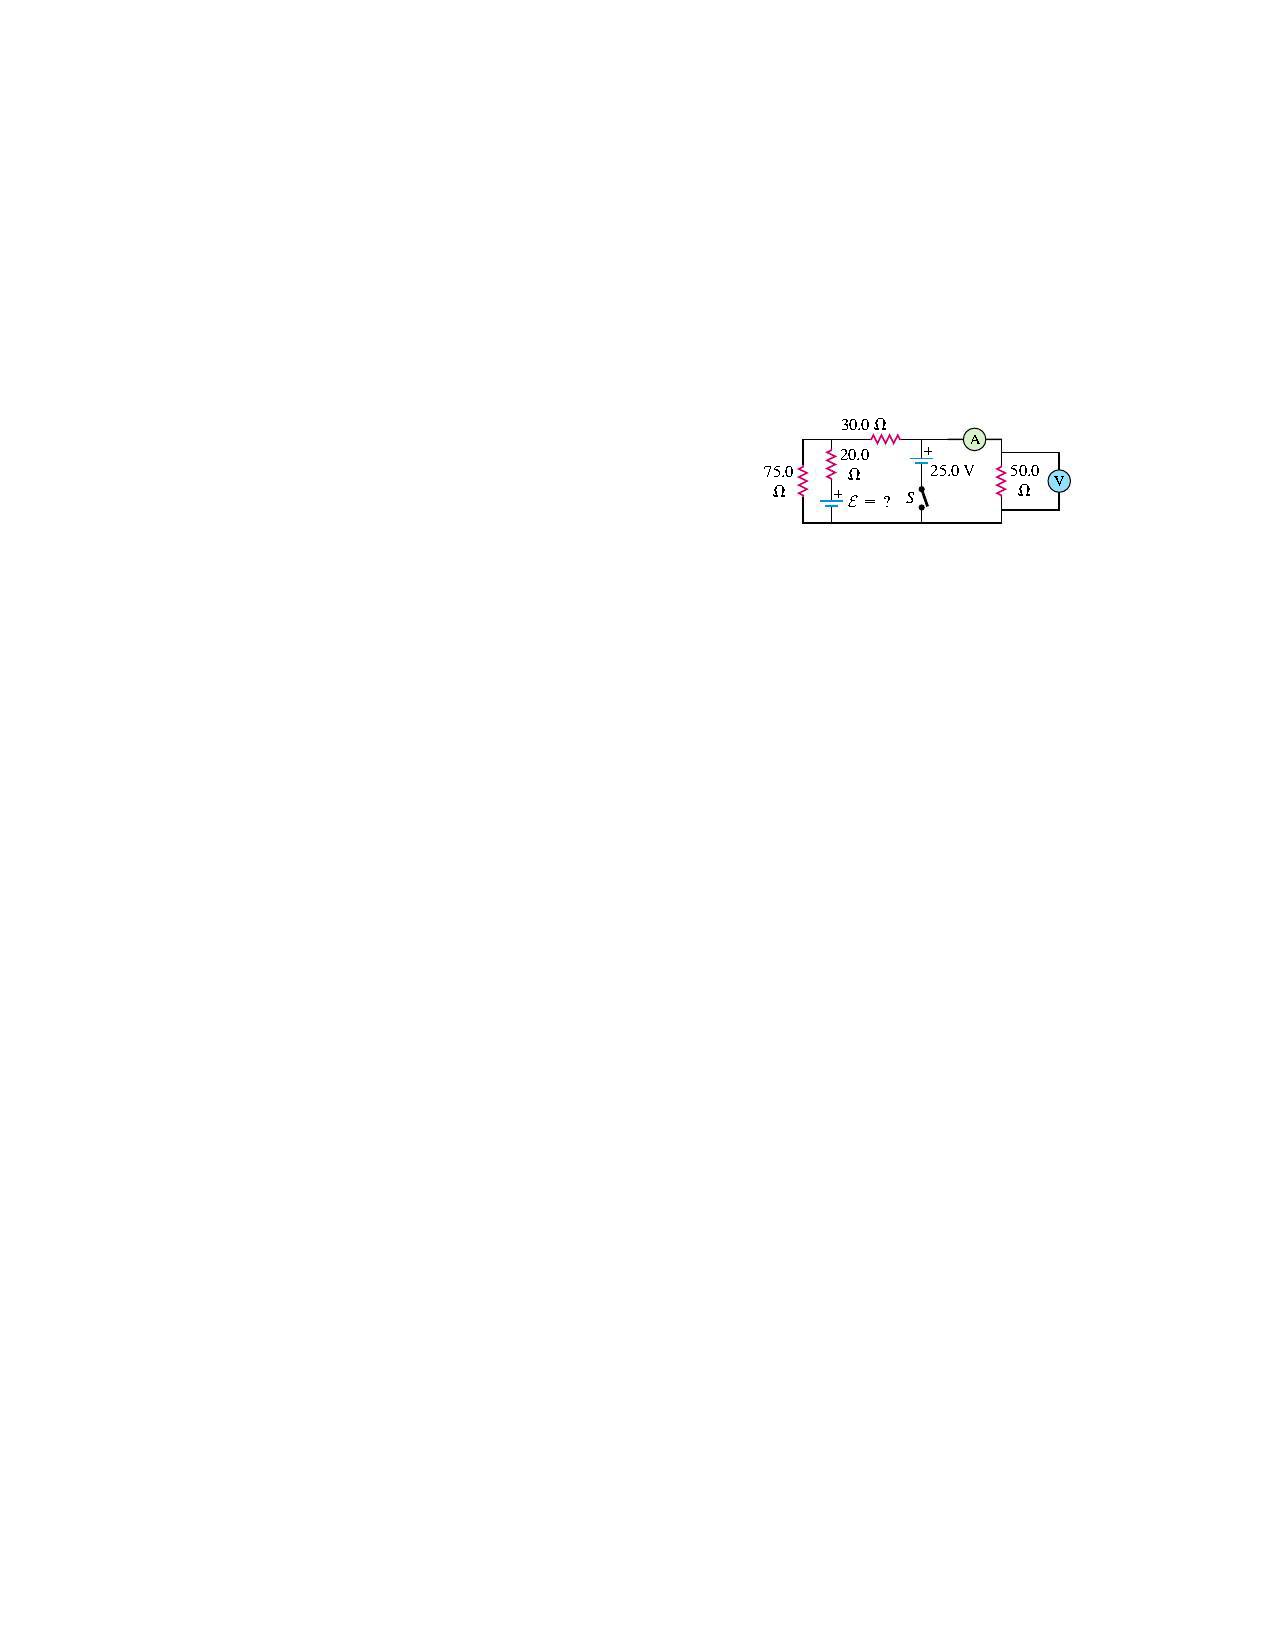
\includegraphics{E26-29}
	\center \textbf{Figure E26.29}
\end{minipage}



\clearpage

\newcommand{\Qo}{Q_0}
\newcommand{\Vo}{V_0}
\newcommand{\Ceq}{C_\text{eq}}
\newcommand{\Req}{R_\text{eq}}

\begin{minipage}[l]{0.75\textwidth}
\paragraph{Exercise 26.41}
\begin{problem}
	In the circuit shown in \textbf{Fig.~E26.41} both capacitors are initially charged to \SI{45.0}{\volt}. \medskip
	\begin{enumerate}
		\item How long after closing the switch $S$ will the potential across each capacitor be reduced to \SI{10.0}{\volt}, and \medskip
		\item what will be the current at that time? \medskip
	\end{enumerate}
\end{problem}
\end{minipage}%
\hspace{0.05\textwidth}%
\begin{minipage}{0.2\textwidth}
	\center 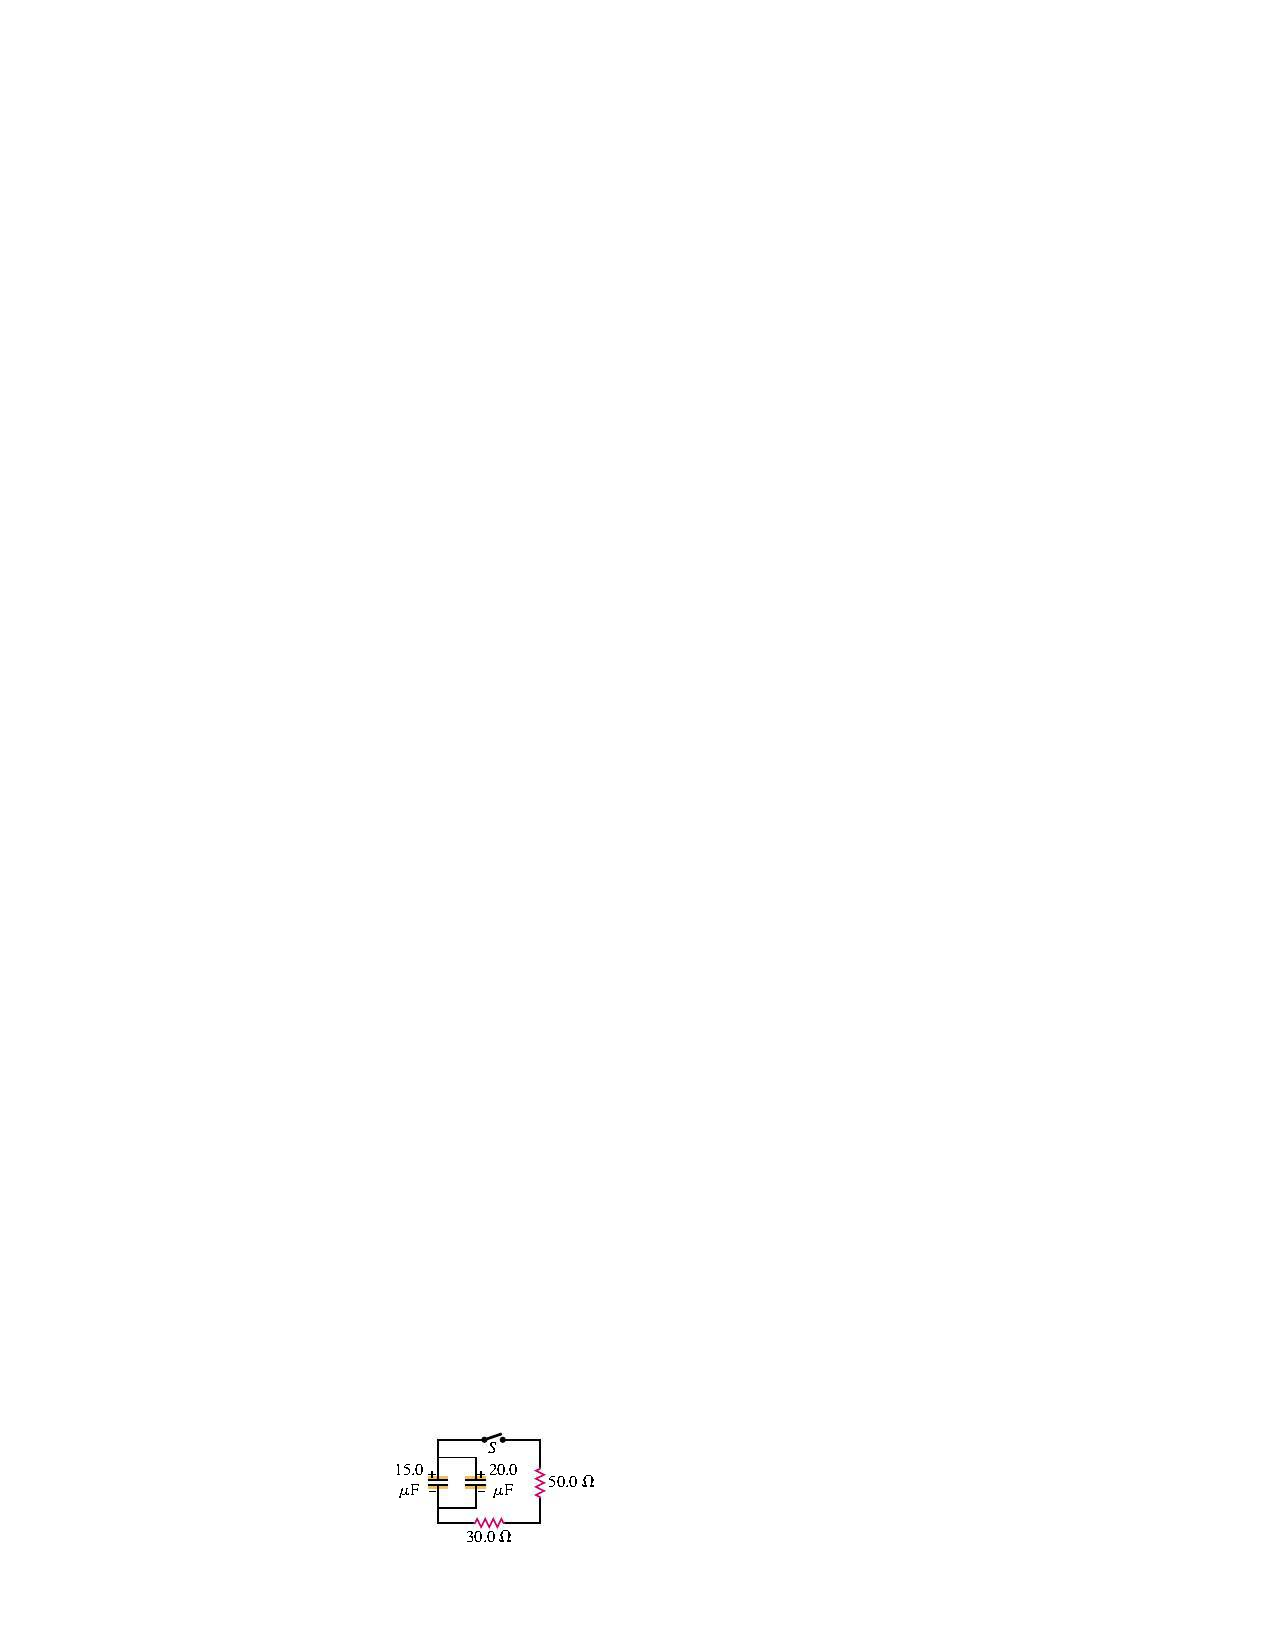
\includegraphics{E26-41}
	\center \textbf{Figure E26.41}
\end{minipage}

\begin{solution}
	This problem is about discharging capacitors.  The charge $q$ on a capacitor at a given time $t$ after an RC circuit is closed is given by
	\beqn \label{26.16} \tag{26.16}
		q = \Qo e^{-t / RC},
	\eeqn
	where $\Qo$ is the initial charge on the capacitor, $C$ is its capacitance, and $R$ is the resistance of the resistor connected in series.
	
	\begin{enumerate}
		\item The definition of capacitance $C$ is
		\beqn \tag{24.1}
			C = \frac{Q}{\Vab},
		\eeqn
		where $Q$ is the charge on the capacitor and $\Vab$ is the potential across it.  $C$ is a property of a given capacitor and does not change with time.  So we can use $Q = C V$ and the fact that $C$ is constant to write \refeq{26.16} in terms of $C$ and $V$:
		\beqn \tag{$*$} \label{Vt}
			v = \Vo e^{-t / RC},
		\eeqn
		where $v$ is the potential across the capacitor at time $t$ after the circuit is closed.
		
		The capacitors in this problem are connected in parallel, so their equivalent capacitance is simply the sum of their individual capacitances:
		\beq
			\Ceq = \SI{15.0}{\micro\farad} + \SI{20.0}{\micro\farad}
			= \SI{35.0}{\micro\farad}.
		\eeq
		The resistors are connected in series, so their equivalent resistance is also just the sum:
		\beq
			\Req = \SI{30.0}{\ohm} + \SI{50.0}{\ohm}
			= \SI{80.0}{\ohm}.
		\eeq
		We can plug these values and our intended value of $v = \Svolt{10.0}$ into \refeq{Vt} to solve for the time $t$:
		\begin{align*}
			\Svolt{10.0} &= (\Svolt{45.0}) \exp(-\frac{t}{(\SI{80.0}{\ohm}) (\SI{35.0}{\micro\farad})})
			\implies
			\frac{2}{9} = \exp(-\frac{t}{\SI{2800}{\micro\second}})
			\implies
			-1.50 = -\frac{t}{\SI{2800}{\micro\second}} \\
			&\implies
			t = \SI{4210}{\micro\second}
			= {\color{blue} \SI{4.21}{\milli\second}},
		\end{align*}
		where we have used the fact that $\SI{1}{\second} = \SI{1}{\ohm\farad}$.
		
		\item The current $i$ through a capacitor at a given time $t$ after the circuit is closed is given by
		\beq \tag{26.13}
			i = \frac{\Qo}{RC} e^{-t / RC}.
		\eeq
		From (a), we know that $\Qo / C = \Vo$, so we can write this as
		\beq
			i = \frac{\Vo}{R} e^{-t / RC}.
		\eeq
		Plugging in our $\Vo$, $\Req$, $\Ceq$, and $t$ that we found in (a), we have
		\beq
			i = \frac{\Svolt{45.0}}{\SI{80.0}{\ohm}} \exp(-\frac{\SI{4210}{\micro\second}}{\SI{2800}{\micro\second}})
			= \frac{9}{16} e^{-1.50}\,\si{\ampere}
			= \frac{9}{16} \frac{2}{9}\,\si{\ampere}
			= \frac{1}{8}\,\si{\ampere}
			= {\color{blue} \SI{0.125}{\ampere}}.
		\eeq
	\end{enumerate}
\end{solution}



\clearpage

\begin{minipage}[l]{0.55\textwidth}
\paragraph{Exercise 26.47}
\begin{problem}
	In the circuit shown in \textbf{Fig.~E26.47} the capacitors are initially uncharged, the battery has no internal resistance, and the ammeter is idealized.  Find the ammeter reading \medskip
	\begin{enumerate}
		\item just after the switch $S$ is closed, and \medskip
		\item after $S$ has been closed for a very long time.
	\end{enumerate}
\end{problem}
\end{minipage}%
\hspace{0.05\textwidth}%
\begin{minipage}{0.4\textwidth}
	\center 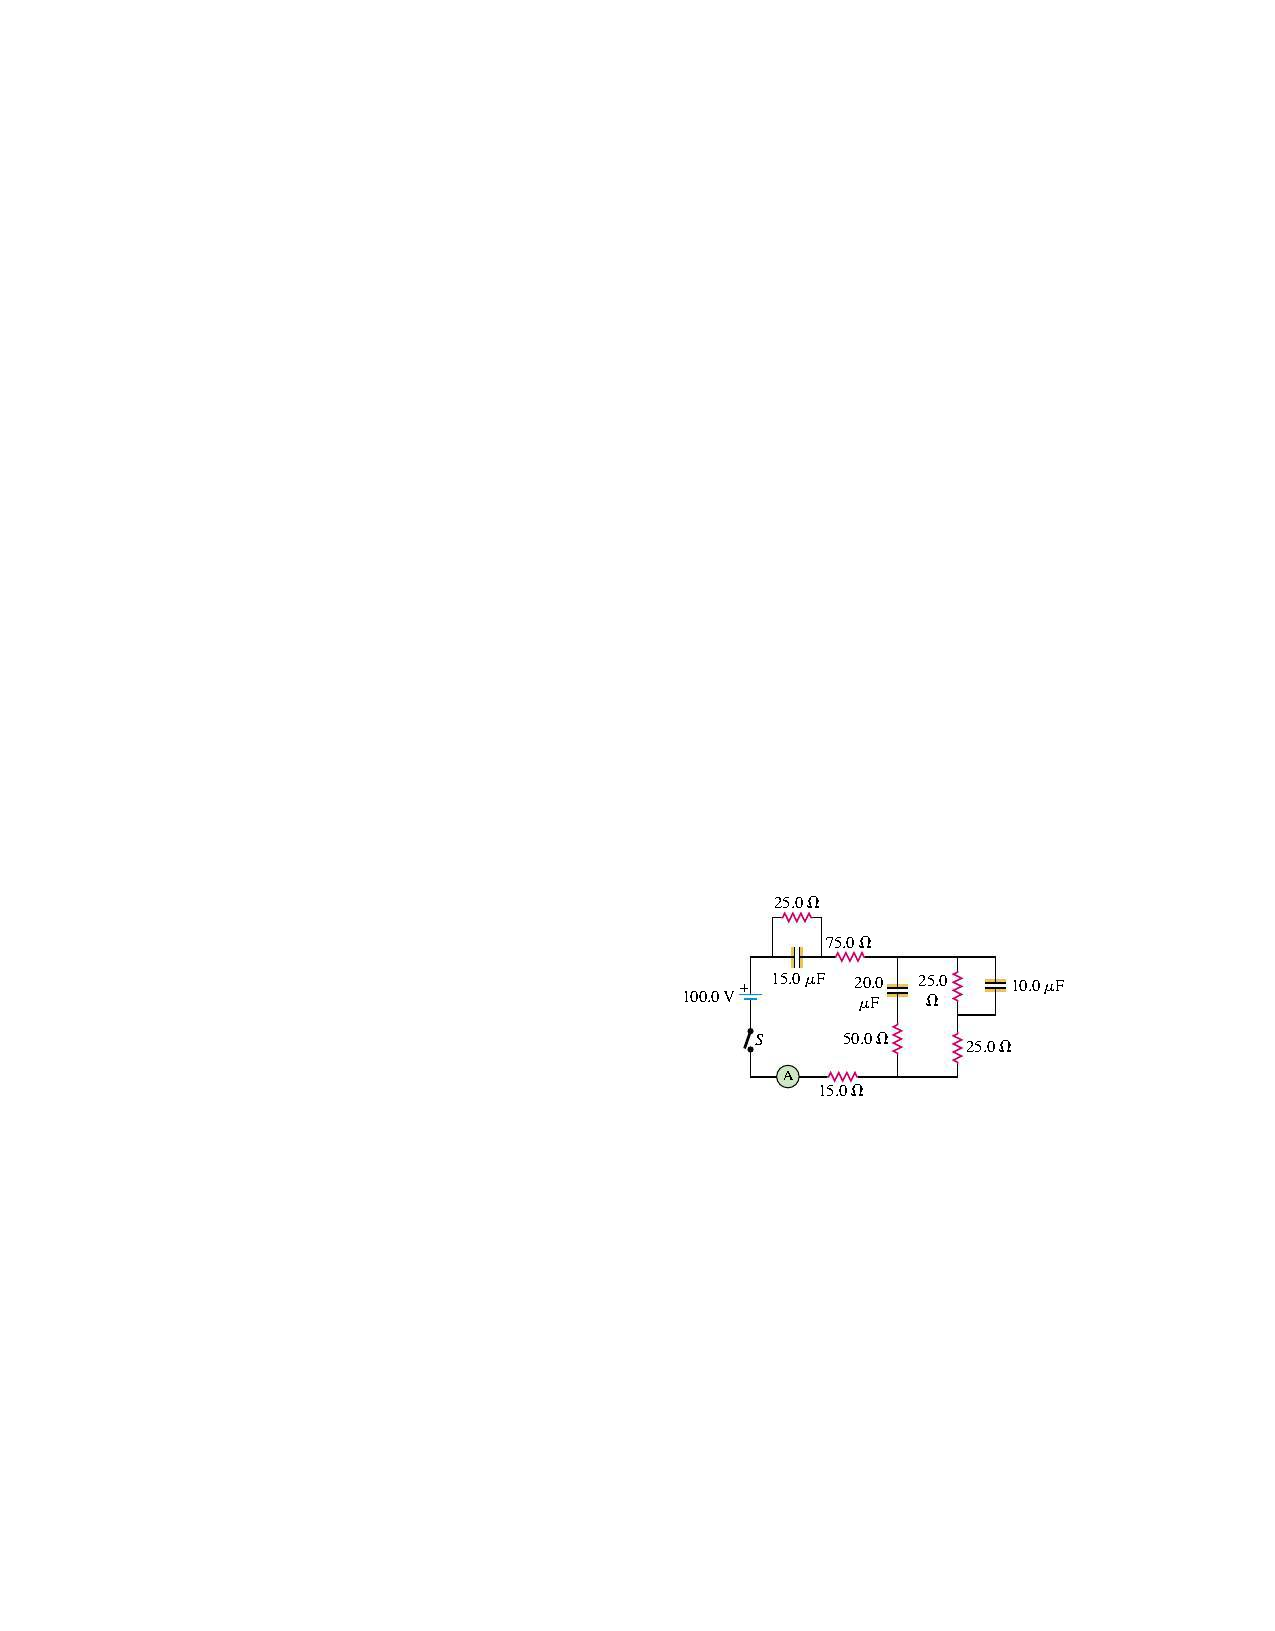
\includegraphics[scale=.31]{E26-47}
	\center \textbf{Figure E26.47}
\end{minipage}



\clearpage

\newcommand{\PcE}{P_\cE}
\newcommand{\dt}{\dd{t}}
\newcommand{\PR}{P_R}
\newcommand{\intoi}{\int_0^\infty}
\newcommand{\UC}{U_C}
\newcommand{\UcE}{U_\cE}
\newcommand{\UR}{U_R}

\paragraph{Problem 26.53}
\begin{problem}
	A capacitor with capacitance $C$ is connected in series to a resistor of resistance $R$ and a battery with emf $\cE$.  The circuit is completed at time $t = 0$.
	\begin{enumerate}
		\item In terms of $\cE$, $R$, and $C$, how much energy is stored in the capacitor when it is fully charged?
		\item The power output of the battery is $\PcE = \cE i$, with $i$ given by Eq.~\refeq{26.13}.  The electrical energy supplied in an infinitesimal time $\dt$ is $\PcE \dt$.  Integrate from $t = 0$ to $t \to \infty$ to find the total energy supplied by the battery.
		\item The rate of consumption of electrical energy in the resistor is $\PR = i^2 R$.  In an infinitesimal time interval $\dt$, the amount of electrical energy consumed by the resistor is $\PR \dt$.  Integrate from $t = 0$ to $t \to \infty$ to find the total energy consumed by the resistor.
		\item What fraction of the total energy supplied by the battery is stored in the capacitor?  What fraction is consumed in the resistor?
	\end{enumerate}
\end{problem}

\begin{solution}
	\begin{enumerate}
		\item In general, the potential energy $U$ stored in a capacitor is given by
		\beqn \tag{24.9}
			U = \frac{1}{2} C V^2,
		\eeqn
		where $C$ is the capacitor's capacitance and $V$ the potential difference between its plates.  When the capacitor its fully charged, the potential difference between its plates is the emf $\cE$.  So we have
		{\color{blue} \beq
			\UC = \frac{1}{2} C \cE^2.
		\eeq }
	
		\item In terms of the given quantities $\cE$, $R$, and $C$, the instantaneous current $i$ is given by
		\beq \label{26.13} \tag{26.13}
			i = \frac{\cE}{R} e^{-t / RC}.
		\eeq
		Plugging this in and integrating, the total energy supplied by the battery is
		\beq
			\UcE = \intoi \PcE \dt
			= \intoi \cE i \dt
			= \intoi \cE \frac{\cE}{R} e^{-t / RC} \dt
			= \frac{\cE^2}{R} \bigg[ - RC e^{-t / RC} \bigg]_0^\infty
			= \frac{\cE^2}{R} R C
			= {\color{blue} C \cE^2}.
		\eeq
		
		\item We just need to plug \refeq{26.13} in again and integrate to find the total energy consumed by the resistor:
		\begin{align*}
			\UR &= \intoi \PR \dt
			= \intoi i^2 R \dt
			= \intoi \left( \frac{\cE}{R} e^{-t / RC} \right)^2 R \dt
			= \frac{\cE^2}{R} \intoi e^{-2t / RC} \dt
			= \frac{\cE^2}{R} \left[ -\frac{RC e^{-2t / RC}}{2} \right]_0^\infty \\
			&= \frac{\cE^2}{R} \frac{RC}{2}
			= {\color{blue} \frac{1}{2} C \cE^2}.
		\end{align*}
		
		\item From (a) and (b), $\UC / \UcE = 1/2$, so {\color{blue} half} of the total energy supplied by the battery is stored in the capacitor.  From (b) and (c), $\UR / \UcE = 1/2$, so the other {\color{blue} half} of the total energy is consumed by the resistor.
	\end{enumerate}
\end{solution}



\clearpage

\begin{minipage}[l]{0.7\textwidth}
\paragraph{Problem 26.59}
\begin{problem}
	Calculate the currents $\Iq$, $\Iw$, and $\Ie$ indicated in the circuit diagram shown in \textbf{Fig.~P26.59}.
\end{problem}
\end{minipage}%
\hspace{0.05\textwidth}%
\begin{minipage}{0.25\textwidth}
	\center 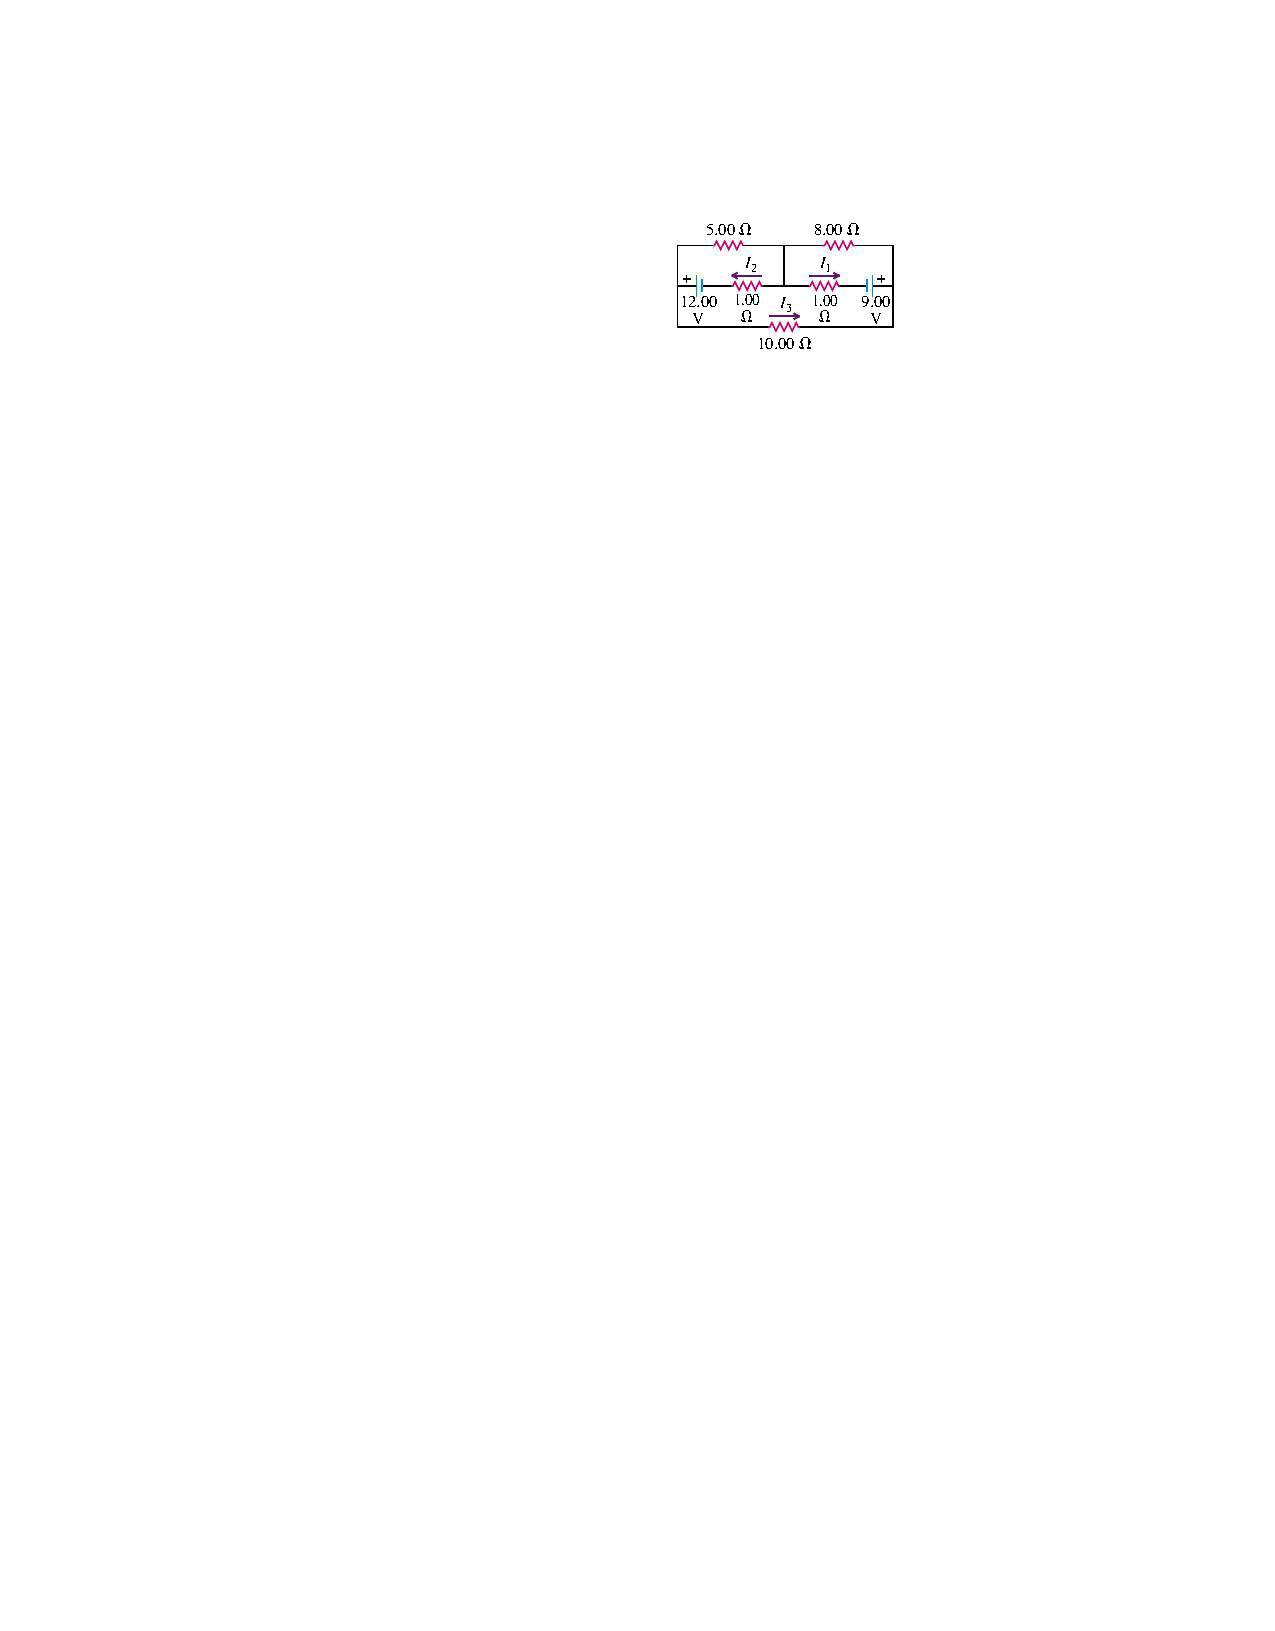
\includegraphics{P26-59}
	\center \textbf{Figure P26.59}
\end{minipage}

\begin{solution}
	This is another problem for Kirchhoff's rules:
	
	\begin{center}
		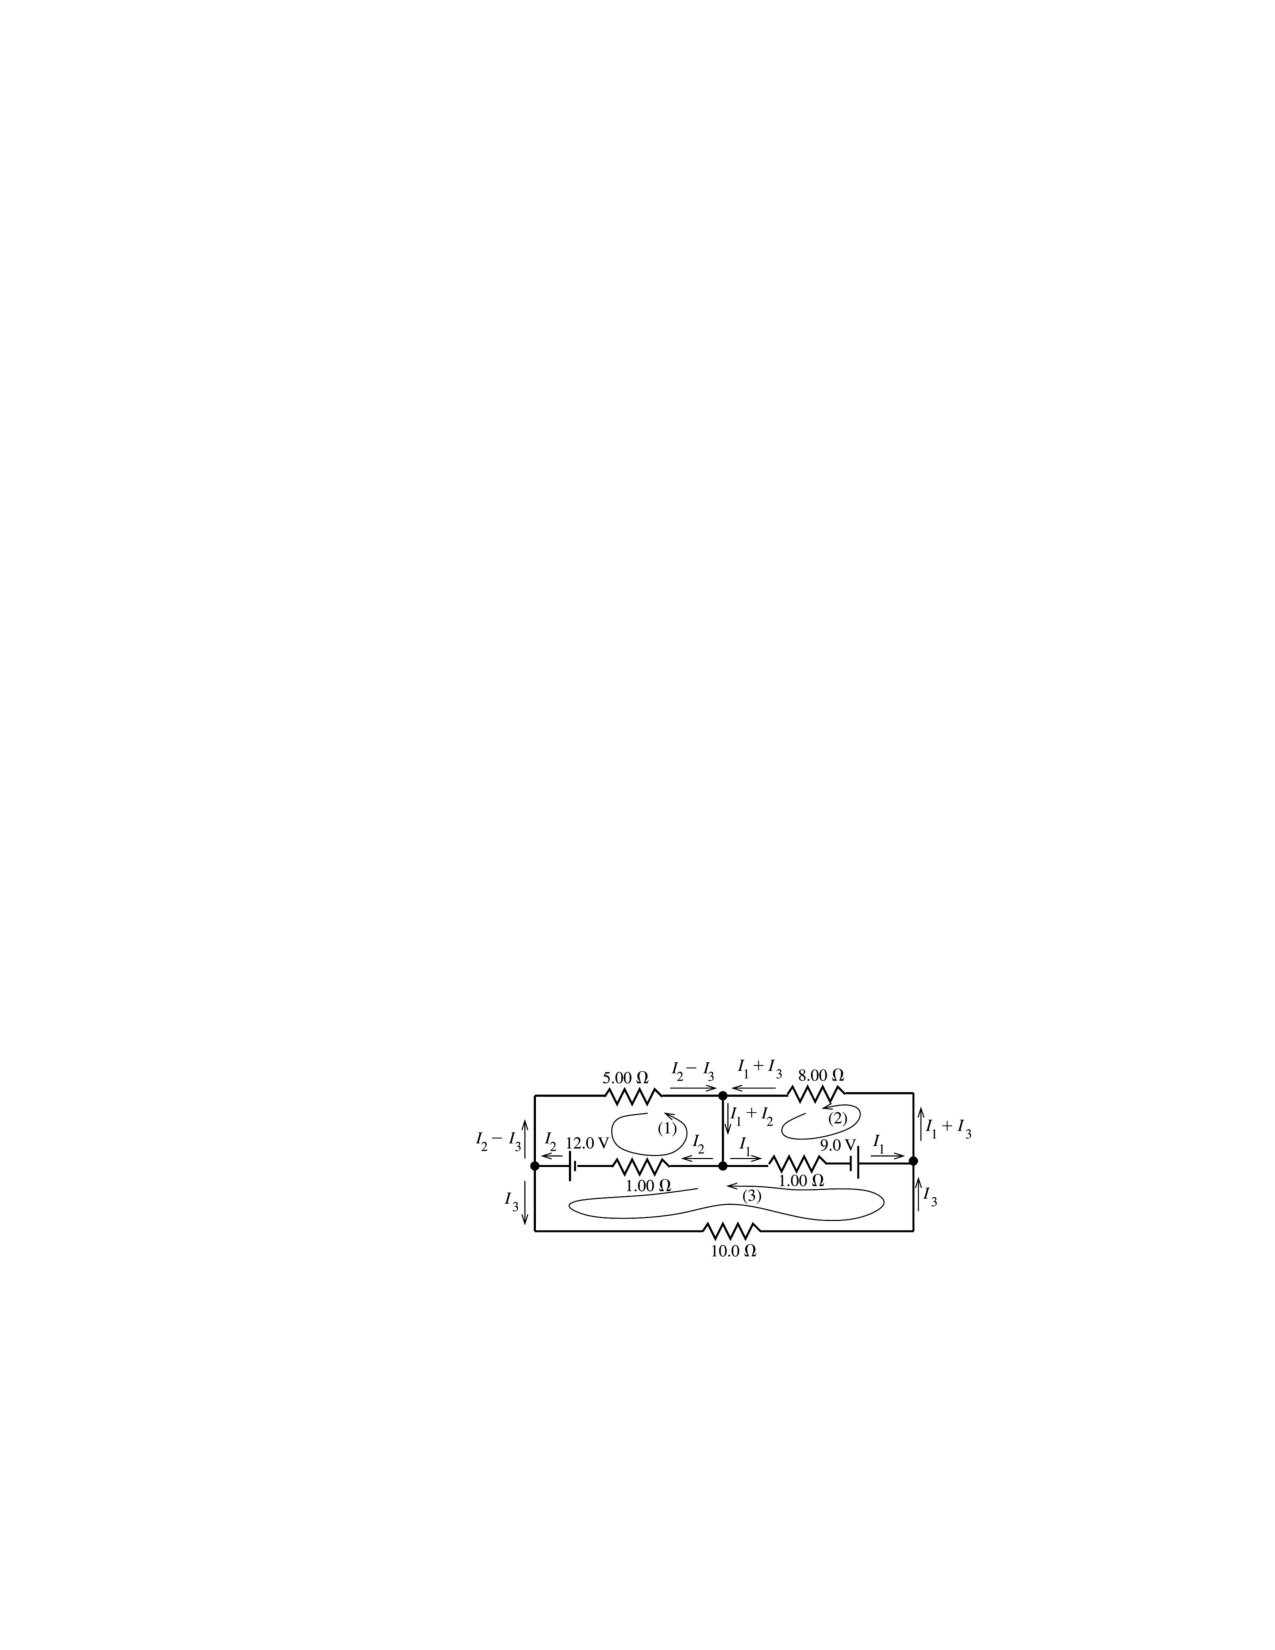
\includegraphics{A26-59}
	\end{center}
	
		The circuit has three loops, so we will need to use the loop rule three times as indicated in the diagram above.  But first we need to use the junction rule to find the current through the \Sohm{5} and \Sohm{8} resistors.  At the junction on the left, we have
	\beq
		0 = \Iw - \Ie + I_{\Sohm{5}}
		\implies
		I_{\Sohm{5}} = \Ie - \Iw,
	\eeq
	meaning it is pointing away from the junction if $\Iw > \Ie$.  At the junction on the right, we have
	\beq
		0 = \Iq + \Ie + I_{\Sohm{8}}
		\implies
		I_{\Sohm{8}} = -\Iq - \Ie,
	\eeq
	meaning it is pointing away from the junction.
	
	Now we can apply the loop rule, moving counterclockwise from each battery.  For loop (1), we have
	\beq
		0 = -\Svolt{12} + (\Sohm{1}) \Iw + (\Sohm{5}) (\Iw - \Ie)
		\implies
		\Samp{12} = 6 \Iw - 5 \Ie.
	\eeq
	For loop (2),
	\beq
		0 = \Svolt{9} - (\Sohm{8}) (\Iq - \Ie) + (\Sohm{1}) \Iq
		\implies
		\Samp{9} = 9 \Iq + 8 \Ie.
	\eeq
	For loop (3), let's start at the \Svolt{12} battery:
	\beq
		0 = \Svolt{12} - (\Sohm{10}) \Ie - \Svolt{9} + (\Sohm{1}) \Iq - (\Sohm{1}) \Iw
		\implies
		\Samp{3} = -\Iq + \Iw + 10 \Ie.
	\eeq
	The matrix equation is
	\beq
		\mqty[ 0 & 6 & -5 \\
			9 & 0 & 8 \\
			-1 & 1 & 10 ]
			\mqty[ \Iq \\ \Iw \\ \Ie ]
			= \mqty[ 12 \\ 9 \\ 3 ],
	\eeq
	which can be solved as follows:
	\beq
		\begin{bmatrix}[c c c | c]
			0 & 6 & -5 & 12 \\
			9 & 0 & 8 & 9 \\
			-1 & 1 & 10 & 3
		\end{bmatrix}
		\sim
		\begin{bmatrix}[c c c | c]
			1 & 0 & 8/9 & 1 \\
			0 & 1 & -5/6 & 2 \\
			-1 & 1 & 10 & 3
		\end{bmatrix}
		\sim
		\begin{bmatrix}[c c c | c]
			1 & 0 & 8/9 & 1 \\
			0 & 1 & -5/6 & 2 \\
			0 & 1 & 98/9 & 4
		\end{bmatrix}
		\sim
		\begin{bmatrix}[c c c | c]
			1 & 0 & 8/9 & 1 \\
			0 & 1 & -5/6 & 2 \\
			0 & 0 & 211/18 & 2
		\end{bmatrix}
		\sim
		\begin{bmatrix}[c c c | c]
			1 & 0 & 0 & 179/211 \\
			0 & 1 & 0 & 452/211 \\
			0 & 0 & 1 & 36/211
		\end{bmatrix}.
		\eeq
		So we have {\color{blue}
		\begin{align*}
			\Iq &= \Samp{0.848} \text{ (to the right)}, &
			\Iw &= \Samp{2.14} \text{ (to the left)}, &
			\Ie &= \Samp{0.171} \text{ (to the right)}.
		\end{align*}}

\end{solution}


\end{document}